\documentclass{article}
\usepackage{geometry}
\usepackage{amsmath}
\usepackage{amssymb}
\usepackage{array}
\usepackage{tabularx}
\usepackage{setspace}
\usepackage{graphicx} % Required for including images
\usepackage{tikz}     % Required for watermarking and shape drawing
\usepackage{fancyhdr} % Required for custom headers/footers
\usepackage{xcolor}
\usepackage{tcolorbox}
\usetikzlibrary{shapes.geometric, arrows, patterns}

\geometry{a4paper, margin=1in}
\setlength{\headheight}{33pt} % Fix header height for logo
\addtolength{\topmargin}{-21pt} % Adjust top margin accordingly

% --- Watermark setup ---
\usepackage{eso-pic}
\newcommand\BackgroundPicture{%
\put(\LenToUnit{0.5\paperwidth},\LenToUnit{0.5\paperheight}){%
\makebox(0,0)[c]{%
\tikz[opacity=0.08]\node{
\includegraphics[width=1\paperwidth]{../oatutors_logo.png}};%
}%
}}
\AddToShipoutPicture{\BackgroundPicture}
% --- End Watermark setup ---

% --- Header setup for logo ---
\pagestyle{fancy}
\fancyhf{} % Clear all header and footer fields
\fancyhead[L]{
\includegraphics[height=1.0cm]{../oatutors_logo.png}} % Logo on the left (slightly smaller for better proportion)
\fancyhead[C]{\textbf{11+ Non-Verbal Reasoning - Extension Activity Sheet}} % Course title in center
\fancyhead[R]{\rightmark} % Section title on the right
\fancyfoot[C]{\thepage} % Page number in the footer
\renewcommand{\headrulewidth}{0.4pt} % Line under the header
\renewcommand{\footrulewidth}{0.4pt} % Line over the footer
% --- End Header setup ---

\begin{document}
\onehalfspacing

\begin{center}
\textbf{\Large Extension Activities: Shape Puzzles}\\
\textbf{\large When You've Finished Early...}
\vspace{0.2cm}
\end{center}

\hrule
\vspace{0.1cm}

\textbf{Name:} \underline{\hspace{4cm}} \quad \textbf{Date:} \underline{\hspace{3cm}} \quad \textbf{Class:} \underline{\hspace{2cm}} \\
\textbf{Lesson Topic:} Collecting \& Disappearing Rules - Extension Activities \\
\textbf{Website:} \texttt{https://oatutors.co.uk/}

\vspace{0.2cm}
\hrule
\vspace{0.3cm}

\begin{tcolorbox}[colback=purple!5,colframe=purple!60,title=Teacher Instructions]
\textbf{Purpose:} These activities develop advanced NVR skills for early finishers.\\
\textbf{Time:} 5-20 minutes depending on activity chosen\\
\textbf{Skills:} Visual processing, logical reasoning, pattern recognition\\
\textbf{Materials:} Colored pencils helpful for some activities
\end{tcolorbox}

\section{Quick Visual Challenges (5-10 minutes)}

\subsection*{Challenge 1: Speed Sorting}
Sort these mixed shapes into groups. How many different ways can you group them?

\begin{center}
\begin{tikzpicture}[scale=0.6]
    % Mixed shapes
    \fill[red] (0,0) circle (0.3);
    \fill[blue] (1,0) rectangle (1.5,0.5);
    \fill[green] (2.5,0) -- (2.8,0.5) -- (3.1,0) -- cycle;
    \fill[red] (4,0) rectangle (4.5,0.5);
    \fill[yellow] (5.5,0) circle (0.3);
    \fill[blue] (6.5,0) circle (0.3);
    \fill[green] (7.5,0) rectangle (8,0.5);
    \fill[red] (9,0) -- (9.3,0.5) -- (9.6,0) -- cycle;
    \fill[yellow] (10.5,0) -- (10.8,0.5) -- (11.1,0) -- cycle;
\end{tikzpicture}
\end{center}

\textbf{Grouping 1 (by shape):} \underline{\hspace{8cm}}

\textbf{Grouping 2 (by color):} \underline{\hspace{8cm}}

\textbf{Grouping 3 (your idea):} \underline{\hspace{8cm}}

\subsection*{Challenge 2: Pattern Detective}
Find the pattern and draw the missing shape:

\begin{center}
\begin{tikzpicture}[scale=0.8]
    % Pattern sequence
    \draw (0,0) rectangle (1.5,1);
    \fill[red] (0.3,0.3) circle (0.2);
    \node at (0.75,-0.3) {1};
    
    \draw (2,0) rectangle (3.5,1);
    \fill[blue] (2.3,0.3) rectangle (2.8,0.7);
    \node at (2.75,-0.3) {2};
    
    \draw (4,0) rectangle (5.5,1);
    \fill[red] (4.3,0.3) circle (0.2);
    \fill[red] (4.8,0.3) circle (0.2);
    \node at (4.75,-0.3) {3};
    
    \draw (6,0) rectangle (7.5,1);
    \fill[blue] (6.3,0.3) rectangle (6.8,0.7);
    \fill[blue] (6.9,0.3) rectangle (7.4,0.7);
    \node at (6.75,-0.3) {4};
    
    \draw (8,0) rectangle (9.5,1);
    \node at (8.75,0.5) {?};
    \node at (8.75,-0.3) {5};
\end{tikzpicture}
\end{center}

\subsection*{Challenge 3: Shape Transformation}
Show what happens when these shapes meet:

\begin{enumerate}
    \item \begin{tikzpicture}[baseline=-0.1cm,scale=0.4]
        \fill[red] (0,0) circle (0.2);
        \fill[red] (0.5,0) circle (0.2);
        \fill[red] (1,0) circle (0.2);
        \node at (1.5,0) {+};
        \fill[blue] (2,0) rectangle (2.3,0.3);
        \fill[blue] (2.5,0) rectangle (2.8,0.3);
        \node at (3.2,0) {=};
    \end{tikzpicture} \underline{\hspace{3cm}}
    
    \item \begin{tikzpicture}[baseline=-0.1cm,scale=0.4]
        \fill[green] (0,0) -- (0.2,0.3) -- (0.4,0) -- cycle;
        \fill[green] (0.6,0) -- (0.8,0.3) -- (1,0) -- cycle;
        \fill[green] (1.2,0) -- (1.4,0.3) -- (1.6,0) -- cycle;
        \fill[green] (1.8,0) -- (2,0.3) -- (2.2,0) -- cycle;
        \node at (2.6,0) {+};
        \fill[yellow] (3,0) circle (0.2);
        \fill[yellow] (3.4,0) circle (0.2);
        \node at (3.8,0) {=};
    \end{tikzpicture} \underline{\hspace{3cm}}
\end{enumerate}

\section{Puzzle Adventures (10-15 minutes)}

\subsection*{Adventure 1: The Magic Box}
This magic box changes shapes according to secret rules. Study the examples and predict what comes out:

\begin{center}
\begin{tikzpicture}[scale=0.8]
    % Magic box
    \draw[thick] (3,1) rectangle (5,3);
    \node at (4,2) {\textbf{MAGIC}};
    \node at (4,1.5) {\textbf{BOX}};
    
    % Example 1
    \draw (0,2.5) rectangle (1.5,3.5);
    \fill[red] (0.3,2.8) circle (0.15);
    \fill[red] (0.7,2.8) circle (0.15);
    \fill[red] (1.1,2.8) circle (0.15);
    
    \draw[->, thick] (1.5,3) -- (3,3);
    \draw[->, thick] (5,3) -- (6.5,3);
    
    \draw (6.5,2.5) rectangle (8,3.5);
    \fill[blue] (6.8,2.8) rectangle (7.2,3.2);
    \fill[blue] (7.3,2.8) rectangle (7.7,3.2);
    
    % Example 2
    \draw (0,1) rectangle (1.5,2);
    \fill[green] (0.5,1.3) -- (0.7,1.7) -- (0.9,1.3) -- cycle;
    \fill[green] (1.1,1.3) -- (1.3,1.7) -- (1.5,1.3) -- cycle;
    
    \draw[->, thick] (1.5,1.5) -- (3,1.5);
    \draw[->, thick] (5,1.5) -- (6.5,1.5);
    
    \draw (6.5,1) rectangle (8,2);
    \fill[purple] (6.8,1.3) circle (0.2);
    
    % Question
    \draw (0,-0.5) rectangle (1.5,0.5);
    \fill[yellow] (0.3,0) rectangle (0.6,0.3);
    \fill[yellow] (0.7,0) rectangle (1,0.3);
    \fill[yellow] (1.1,0) rectangle (1.4,0.3);
    \fill[yellow] (0.5,-0.2) rectangle (0.8,0.1);
    
    \draw[->, thick] (1.5,0) -- (3,0);
    \draw[->, thick] (5,0) -- (6.5,0);
    
    \draw (6.5,-0.5) rectangle (8,0.5);
    \node at (7.25,0) {\textbf{?}};
\end{tikzpicture}
\end{center}

What do you think the rule is? \underline{\hspace{6cm}}

Draw your answer in the box above.

\subsection*{Adventure 2: Shape Sudoku}
Fill in the grid so each row and column contains exactly one of each shape:

\begin{center}
\begin{tikzpicture}[scale=0.8]
    % Grid
    \draw (0,0) grid (3,3);
    
    % Given shapes
    \fill[red] (0.5,2.5) circle (0.2);
    \fill[blue] (1.5,2.3) rectangle (1.8,2.7);
    \fill[green] (2.2,1.5) -- (2.5,1.8) -- (2.8,1.5) -- cycle;
    \fill[blue] (0.3,1.3) rectangle (0.7,1.7);
    \fill[green] (1.2,0.5) -- (1.5,0.8) -- (1.8,0.5) -- cycle;
    
    % Legend
    \node at (4,2.5) {Shapes to use:};
    \fill[red] (4.5,2) circle (0.2);
    \fill[blue] (4.3,1.3) rectangle (4.7,1.7);
    \fill[green] (4.2,0.5) -- (4.5,0.8) -- (4.8,0.5) -- cycle;
\end{tikzpicture}
\end{center}

\subsection*{Adventure 3: The Disappearing Act}
Design your own magic trick where shapes disappear and reappear:

\textbf{Step 1:} Start with these shapes: \underline{\hspace{6cm}}

\textbf{Step 2:} Add these shapes: \underline{\hspace{6cm}}

\textbf{Step 3:} Result after magic: \underline{\hspace{6cm}}

\textbf{Explain your magic trick:} \underline{\hspace{8cm}}

\section{Creative Challenges (15-20 minutes)}

\subsection*{Creative Challenge 1: Shape Art}
Create a picture using only the basic shapes (circles, squares, triangles). Your picture should tell a story about the collecting and disappearing rules.

\vspace{6cm}

\textbf{Story about your picture:} \underline{\hspace{8cm}}

\subsection*{Creative Challenge 2: Invent New Rules}
Imagine you could create new rules for shape puzzles. What would they be?

\textbf{New Rule 1:} \underline{\hspace{8cm}}

\textbf{Example:} \underline{\hspace{8cm}}

\textbf{New Rule 2:} \underline{\hspace{8cm}}

\textbf{Example:} \underline{\hspace{8cm}}

\subsection*{Creative Challenge 3: Shape Language}
Invent a secret code using shapes. Write your name in shape code:

\textbf{My code key:}
\begin{itemize}
    \item A = \underline{\hspace{1cm}} \quad B = \underline{\hspace{1cm}} \quad C = \underline{\hspace{1cm}} \quad D = \underline{\hspace{1cm}}
    \item E = \underline{\hspace{1cm}} \quad F = \underline{\hspace{1cm}} \quad G = \underline{\hspace{1cm}} \quad H = \underline{\hspace{1cm}}
\end{itemize}

\textbf{My name in shape code:}

\vspace{2cm}

\section{Brain Teasers (For Advanced Students)}

\subsection*{Teaser 1: The Ultimate Puzzle}
You have a box with 100 red circles, 100 blue squares, and 100 green triangles. You can only take out shapes in groups that follow the collecting and disappearing rules. What's the minimum number of steps to empty the box completely?

\textbf{My strategy:}
\vspace{3cm}

\textbf{Number of steps:} \underline{\hspace{3cm}}

\subsection*{Teaser 2: The Pattern Master}
Create a 6-step pattern where:
- Steps 1-3 follow one rule
- Steps 4-6 follow a different rule
- The final result is exactly 2 shapes

\textbf{Your pattern:}
\vspace{4cm}

\subsection*{Teaser 3: The Reverse Engineer}
If the final result is 5 blue circles and 3 red squares, and you know that 4 green triangles were added at some point, what could the starting position have been?

\textbf{Possible starting position:} \underline{\hspace{6cm}}

\textbf{Show your working:}
\vspace{3cm}

\section{Investigation Corner}

\subsection*{Investigation 1: Real-World Connections}
Where might you see collecting and disappearing rules in real life? Think about:
- Games you play
- Things in nature  
- Computer programs
- Sports

\textbf{Real-world example 1:} \underline{\hspace{6cm}}

\textbf{How it's similar:} \underline{\hspace{8cm}}

\textbf{Real-world example 2:} \underline{\hspace{6cm}}

\textbf{How it's similar:} \underline{\hspace{8cm}}

\subsection*{Investigation 2: Mathematical Thinking}
The collecting and disappearing rules are similar to math operations. Can you make connections?

\textbf{Collecting rule is like:} \underline{\hspace{6cm}}

\textbf{Disappearing rule is like:} \underline{\hspace{6cm}}

\textbf{What math topic could help with shape puzzles?} \underline{\hspace{6cm}}

\section{Design Your Own Challenge}

Create a puzzle for a friend that uses everything you've learned:

\textbf{Your puzzle title:} \underline{\hspace{6cm}}

\textbf{Your puzzle:}
\vspace{4cm}

\textbf{The answer:} \underline{\hspace{6cm}}

\textbf{Test it on a friend! Did they get it right?} $\square$ Yes $\square$ No

\section*{Reflection Zone}

\textbf{Which activity made you think the hardest?} \underline{\hspace{6cm}}

\textbf{What new idea did you discover?} \underline{\hspace{8cm}}

\textbf{If you could teach someone about shape puzzles, what would you tell them?}

\underline{\hspace{10cm}}

\textbf{What shape puzzle would you like to explore next?} \underline{\hspace{6cm}}

\vspace{1cm}

\begin{tcolorbox}[colback=orange!10,colframe=orange!60,title=Teacher Assessment Notes]
\textbf{Student demonstrated:}
$\square$ Advanced visual processing skills\\
$\square$ Creative problem-solving approach\\
$\square$ Logical reasoning development\\
$\square$ Pattern recognition mastery\\
$\square$ Independent investigation skills\\

\textbf{Areas for further development:} \underline{\hspace{8cm}}

\textbf{Recommended next NVR topics:} \underline{\hspace{8cm}}
\end{tcolorbox}

\end{document}